\section{Sucesiones}

\begin{definicion}
	Una sucesión es cualquier función cuyo dominio es un conjunto infinito contable, i.e. $\mathbb{Z}^+, \mathbb{N},\mathbb{Q}$. 
\end{definicion}

\begin{ejemplo}
	$f:\mathbb{Z}^+\to\mathbb{R}\ni f(n)=\sen n$ es una sucesión. 
\end{ejemplo}

\begin{definicion}
	Se dice que la sucesión $(a_n)$ converge al número $l$, denotado $a_n\to l$, si $\forall \varepsilon >0\exists N\in\mathbb{Z}^+\ni$ si $n\geq N\implies |a_n-l|<\varepsilon$. 
\end{definicion}
\begin{nota}
	Si existe $l$, entonces es el límite de $(a_n)$. Notación: $$\lim_{n\to\infty} a_n=l.$$
\end{nota}

\begin{ejemplo}
	Compruebe que $\lim_{n\to\infty}\frac{1}{n}=0$. 
	\begin{center}
		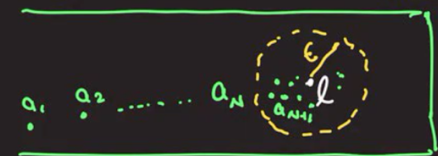
\includegraphics[scale=0.4]{images/4/1}
	\end{center}
\end{ejemplo}
\begin{sol}
	Dado $\varepsilon>0\exists N=\underline{1/\varepsilon}\in \mathbb{Z}^+\ni $ si $n\geq N\implies \left|\frac{1}{n}-0\right|<\varepsilon\implies \left|\frac{1}{n}-0\right|=\left|\frac{1}{n}\right|=\frac{1}{n}<\varepsilon\implies n>\frac{1}{\varepsilon}$.
\end{sol}

\begin{teorema}
	El límite de una sucesión, si existe, es único. 
\end{teorema}
\begin{proof}
	Suponemos que $a_n\to l$ y $a_n\to l'$. 
	\begin{enumerate}
		\item Como $a_n\to l\implies$ Dado $\varepsilon >0\exists N_1\in \mathbb{Z}^+\ni$ si $n\geq N_1\implies |a_n-l|<\varepsilon/2$. 
		\item Como $a_n\to l'\exists N_2\in \mathbb{Z}^+\ni$ si $n\geq N_2$, entonces $|a_n-l|'<\varepsilon/2$.
		\item Sea $N=\max\{N_1,N_2\}\implies$ para $n\geq N$, se cumple: 
		$$|l-l'|=|l-a_n+a_n-l'|=|(l-a_n)+(a_n-l')|\leq \underbrace{|l-a_n|}_{|a_n-l|}+|a_n-l'|<\varepsilon/2+\varepsilon/2=\varepsilon.$$
		i.e. $|l-l'|<\varepsilon$. Por la arbitrariedad de $\varepsilon \implies l=l'$. 
		\begin{cajita}
			$|l-l'|\leq \inf\{\in: \in >0\}$
		\end{cajita}
	\end{enumerate}
\end{proof}

\begin{teorema}
	Una sucesión convergente es acotada. 
\end{teorema}
\begin{proof}
	Como $a_n\to l\implies$ Dado $\underline{\varepsilon=1}\exists N\in\mathbb{Z}^+\ni$ si $n\geq N\implies |a_n-l|<1$. Entonces, $|a_n|-|l|\leq \left||a_n|-|l|\right|\leq |a_n-l|<1\implies |a_n|-|l|<1\implies |a_n|<|l|+1, \forall n\geq N$. $\implies$ Hagamos $M=\max\{|x_1|,|x_2|,\cdots, |x_{n-1}|, \underbrace{|l|+1}_{|a_n|, \forall n\geq N}\}$. $\implies |a_n|\leq M, \forall n\in \mathbb{Z}^+$. $\implies (a_n)$ es acotada. 
\end{proof}

\begin{teorema}
	Si $a_n\to l\implies |a_n|\to|l|$. 
\end{teorema}

\begin{proof}
	Si $a_n\to l\implies \forall \varepsilon >0\exists N\in Z^+\ni$ si $n\geq N\implies |a_n-l|<\varepsilon$. Por desigualdad triangular: $$\left||a_n|-|l|\right|<|a_n-l|<\varepsilon\implies ||a_n|-|l||<\varepsilon\implies |a_n|\to|l|.$$
\end{proof}

\begin{teorema}
	Sean $(a_n)$ y $(b_n)$ sucesiones convergentes tal que $a_n\to l$ y $b_n\to l'$. Entonces: 
	\begin{enumerate}
		\item $(a_n+b_n)\to l+l'$. 
		\item $(a_n\cdot b_n)\to l\cdot l'$. 
	\end{enumerate}
\end{teorema}
\begin{proof}
	\begin{enumerate}
		\item Sea $\varepsilon>0\implies \exists N_1\in \mathbb{Z}^+ \ni$ Si $n\geq N\implies |a_n-l|<\varepsilon/2\implies \exists N_2\in \mathbb{Z}^+\in$ si $n\geq N_2\implies |b_n-l'|<\varepsilon/2$. 
		Hagamos $N=\max\{N_1,N_2\}$. Entonces, se tiene: 
		$|(a_n+b_n)-(l+l')|=|(a_n-l)+(b_n-l')|\leq |a_n-l|+|b_n-l'|<\varepsilon/2+\varepsilon/2=\varepsilon, \quad \forall n\geq N$. $\implies (a_n+b_n)\to l+l'$. 
		\item \begin{enumerate}
			\item $|a_nb_n-l\cdot l'|= |a_nb_n-a_nl'+a_nl'-l\cdot l'|=|a_n(b_n-l')+(a_n-l)\cdot l'|\leq |a_n(b_n-l')|+|(a_n-l)\cdot l'|=|a_n|\cdot |b_n-l'|+|a_n-l|\cdot |l'|$.
			\item Como $a_n$ es convergente. $\implies a_n$ es acotada. $\implies \exists M'\geq 0 \ni |a_n|\leq M', \forall n\in Z^+$. 
			\item Hagamos $M=\max\{M',|l'|\}$
			\item Como $a_n\to l$ y $b_n\to l'$, entonces $\forall \varepsilon >0$, \begin{enumerate}
				\item $\exists N_1\in \mathbb{Z}^+\ni$ si $n\geq N_1\implies |a_n-l|<\varepsilon$.
				\item $\exists N_2 \in \mathbb{Z}^+\ni$ si $n\geq N_2\implies |b_n-l'|<\varepsilon$. 
			\end{enumerate}
		\item Hacemos $N=\max\{N_1,N_2\}$. Entonces:
		$$|a_n\cdot b_n-l\cdot l'|\leq |a_n|\cdot |b_n-l'|+|a_n-l|\cdot |l'|<M\cdot \frac{\varepsilon}{2M}+\frac{\varepsilon}{2M}M=\varepsilon, n\geq N.$$
		$\implies a_nb_n\to l\cdot l'$. 
		\end{enumerate}
	\end{enumerate}
\end{proof}


\begin{teorema}
	Si $(a_n)$ converge a $l$, $l\neq 0$, entonces $a_n\neq 0$ a partir de algún $N\in\mathbb{Z}^+$ y $$\frac{1}{a_n}\to \frac{1}{l}.$$
\end{teorema}

\begin{proof}
	Por hipótesis: $a_n\to l\implies |a_n|\to |l|$. Sea $\underline{\varepsilon= |l|/2}\implies \exists N\in \mathbb{Z}^+\ni$ si $n\geq N$, entonces $\textcolor{red}{\underbrace{\left||a_n|-|l|\right|}}<|l|/2 \implies -\left(|a_n|-|l|\right)<|l|/2 \implies -|a_n|+|l|<|l|/2 \implies \underbrace{|l|/2<|a_n|}_{1/|a_n|<2/|l|}, \forall n\geq N$. 
	$$\left|\frac{1}{a_n}-\frac{1}{l}\right|=\left|\frac{l-a_n}{a_n\cdot l}\right|=\frac{|l-a_n|}{|a_n|\cdot |l|}=\frac{|a_n-l|}{|a_n|\cdot |l|}<\frac{|a_n-l|(2)}{|l|\cdot |l|}=\frac{2\textcolor{red}{\overbrace{|a_n-l|}}}{den}$$
	$\implies 1/a_n \to 1/l$.
\end{proof}

\begin{teorema}
	\begin{enumerate}
		\item Si $(a_n)$ es una sucesión de términos no negativos $\ni a_n\to l\implies l$ es no negativo. 
		\item Si $a_n\to l$ y $b_n\to l'$, con $a_n\leq b_n, \forall n\in\mathbb{Z}^+\implies l\leq l'$.
	\end{enumerate}
\end{teorema}

\begin{corolario}
	Si $a_n\to l$ y si $\alpha \in\mathbb{R}\implies \alpha a_n\to \alpha l$. 
\end{corolario}

\begin{ejemplo}
	Demuestre que $\lim_{n\to\infty} \frac{n-1}{n+1}=1$.
\end{ejemplo}
\begin{sol}
	Dado $\varepsilon>0\exists N=\underline{2/\varepsilon}\in\mathbb{Z}^+\ni $ si $n\geq N\implies \left|\frac{n-1}{n+1}-1\right|<\varepsilon$.
	$$\left|\frac{n-1}{n+1}-1\right|=\left|\frac{n-1-(n+1)}{n+1}\right|=\left|\frac{-2}{n+1}\right|=\frac{2}{n+1}<\frac{2}{n}<\varepsilon.$$
	$$\implies \frac{n}{2}>\frac{1}{\varepsilon}\implies n>2/\varepsilon.$$
\end{sol}
\begin{ejemplo}
	Compruebe que $\lim_{n\to\infty}\left[\sqrt{n+1}-\sqrt{n}\right]=0$.
\end{ejemplo}
\begin{sol}
	Dado $\varepsilon>0\exists N=\underline{1/(4\varepsilon^2)}\in \mathbb{Z}^+ni$ si $n\geq N\implies \left|\left(\sqrt{n+1}-\sqrt{n}\right)-0\right|<\varepsilon$.
	
	$\implies \left|\sqrt{n+1}-\sqrt{n}\right|=\sqrt{n+1}-\sqrt{n}=\left(\sqrt{n+1}-\sqrt{n}\right)\left(\frac{\sqrt{n+1}+\sqrt{n}}{\sqrt{n+1}+\sqrt{n}}\right)=\frac{(n+1)-n}{\sqrt{n+1}+\sqrt{n}}=\frac{1}{\sqrt{n+1}+\sqrt{n}}<\frac{1}{2\sqrt{n}}<\varepsilon\implies 2\sqrt{n}>1/\varepsilon\implies \sqrt{n}>1/2\varepsilon \implies n>1/(4\varepsilon^2).$ 
\end{sol}
\begin{nota}
	Considere las sucesiones: $a_n=n$ y $b_n=(-1)^n$. Ambas sucesiones divergen (i.e no converge). 
\end{nota}

\begin{definicion}
	Se dice que $(a_n)$ tiende a infinito ($\lim_{n\to\infty}a_n=\infty$), si $\forall M>0\exists n\in\mathbb{Z}^+\ni a_n>M$. 
	\begin{nota}
		La acotación de una sucesión no asegura convergencia. 
	\end{nota}
\end{definicion}

\begin{teorema}
	Suponga $(x_n), (y_n), (z_n)$ son sucesiones de números reales tal que 
	$$x_n\leq y_n\leq z_n, \quad \forall n\in \mathbb{Z}^+.$$
	Si $\lim x_n=\lim z_n\implies (y_n)$ converge y $\lim x_n =\lim y_n=\lim z_n$. 
\end{teorema}

\begin{proof}
 Supóngase que $\lim_{n\to\infty}x_n=\lim_{n\to\infty}z_n=w$. Si $\varepsilon>0\implies \exists N\in \mathbb{Z}^+\ni |x_n-w|<\varepsilon$ y $|z_n-w|<\varepsilon$. 
 \begin{cajita}
 	\begin{enumerate}
 		\item Si $\varepsilon>0\exists N_1\in \mathbb{Z}^+\ni |x_n-w|<\varepsilon, \forall n\geq N_1$. 
 		\item Si $\varepsilon>0\exists N_2\in \mathbb{Z}^+\ni |x_n-w|<\varepsilon, \forall n\geq N_2$. 
 	\end{enumerate}
 $\implies$ Hagamos $N=\max\{N_1,N_2\}$. 
 \end{cajita}
Como $x_n\leq y_n\leq z_n\implies x_n-w\leq y_n-w\leq z_n-w, \ \forall n\in\mathbb{Z}^+$. Nótese que: $-\varepsilon<x_n-w<\varepsilon$, y que: $-\varepsilon<z_n-w<\varepsilon$. $\implies -\varepsilon<x_n-w\leq y_n-w\leq z_n-w<\varepsilon\implies -\varepsilon<y_n-w<\varepsilon \iff |y_n-w|<\varepsilon, \forall n\geq N$. $\implies$ Por la arbitrariedad de $\varepsilon$, $\lim_{n\to\infty}y_n=w$. $\implies \lim_{n\to\infty}x_n=\lim_{n\to\infty}y_n=\lim_{n\to\infty}z_n$. 
\end{proof}

